\documentclass{article}
\usepackage{url}
\usepackage{color}
\usepackage{pdfcolmk}
\usepackage[normalem]{ulem}
\useunder{\uline}{\ul}{}
\usepackage{Sweave}
\begin{document}
\Sconcordance{concordance:hw2_report.tex:hw2_report.Rnw:%
1 6 1 1 0 110 1 1 2 1 0 3 1 1 3 5 0 1 2 148 1}

\DefineVerbatimEnvironment{Sinput}{Verbatim}{formatcom = {\color[rgb]{0, 0, 0.56}}}
\DefineVerbatimEnvironment{Soutput}{Verbatim}{formatcom = {\color[rgb]{0.56, 0, 0}}}
\graphicspath{{/Users/jacquelineroudes/Documents/GTL_courses/Data_Visual_Analytics/Assignments/Homework2}}
\begin{titlepage}
\vspace*{\stretch{1}}

\begin{center}

\includegraphics[scale=0.4]{GT_logo.jpeg}
\end{center}
\vspace*{\stretch{1}}
\hrulefill
\begin{center}\bfseries\huge
   HW2 Report \\
    Data Visualization\\
    \hrulefill
\end{center}
\vspace*{1cm}
\begin{minipage}[t]{0.4\textwidth}
  \begin{flushleft} \large
    \emph{Subject : \\
    CSE 6242 Spring 2017 - OMS}\\
  \end{flushleft}
\end{minipage}
\begin{minipage}[t]{0.6\textwidth}
  \begin{flushright} \large
    \emph{Author :} \\
    Melisande Zonta Roudes \\
    GT account name : mzr3 \\
  \end{flushright}
\end{minipage}
\vspace*{\stretch{2}}
\begin{flushright}
        \today 
\end{flushright} 

\end{titlepage}

\section{Professional Education by State}

The midwest dataset has 437 counties in the midwest region and 28 attributes from which are states, percpof (percentage of professional education) and popadults (percentage of adults in the population).

\paragraph{Relationship between states and percprof}
We will here study the relationship between the states in the Midwest region and the percentage of people that have a professional education. To do so we will use \textbf{Interpretation B}. Indeed we will treat the raw percprof for each county as a metric. We will consider the population adults since they are mainly the people concerned by professional employment.

\begin{figure}[!ht]
\centering
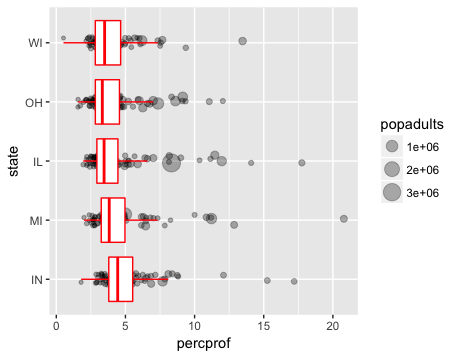
\includegraphics[width=.8\textwidth]{question1.png}
 \caption{Relationship between pecprof and state}
\label{question1}
\end{figure}

This scatter plot superposed on a box plot allows us to determine the order between the median of each state. Wisconsin, Ohio and Illinois have approximately the same median, Michigan has an upper median and Indiana has the maximal median. We can see that they are all below $5\%$ and that the third quartiles are inferior to $6\%$.The spreads are equivalent and there are no disjoint values. The difference between those states stands in outliers. Indeed I removed the outliers of the boxplots to represent the scatter plot with the variation on popadults. We can observe that Michigan has the maximum outlier but it's not a significant one (1e+06) and Wisconsin the minimum value. However the outliers of Illinois show that even if it has the lowest median, it would have the upper mean because we can observe the presence of the county COOK which has a population of 3204947 people. So it's also an element which proves that median is a statistical metric that has more value than mean.

\paragraph{Identification of extreme values}
This way of processing data can't provide us informations on the lowest and highest percentage of adult population with a professional education because it shows data for each state with the values for each counties. However each county has not the same weight in the state so these datas need to be normalized in their state otherwise it is meaningless.

Hence we will use now \textbf{Interpretation A} and apply the formula : 
\begin{equation}
\forall s, percprof_{s} = \frac{\Sigma_{c \in s} percprof_{c} \times popadults_{c}}{ \Sigma_{c \in s} popadults_{c}}
\end{equation}

\begin{figure}[!ht]
\centering
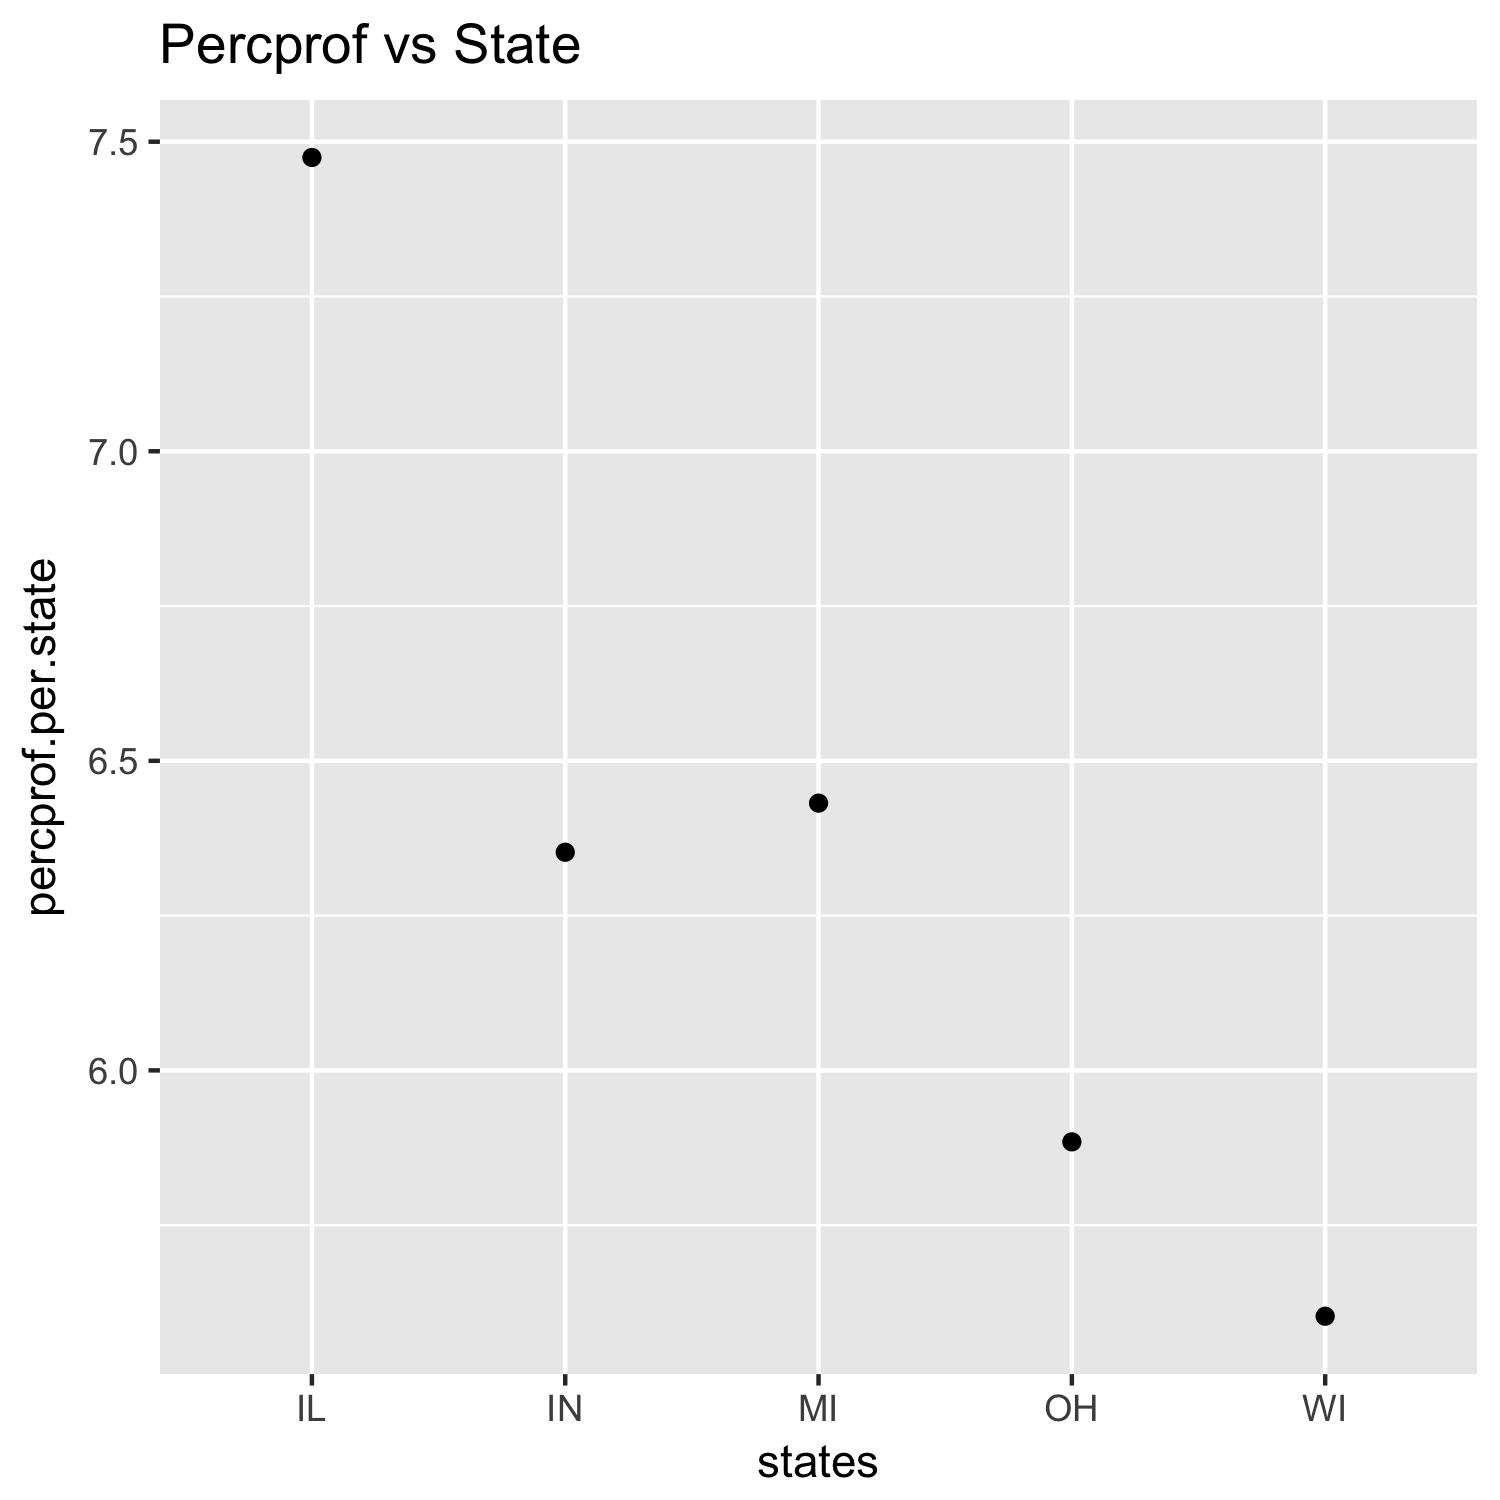
\includegraphics[width=.8\textwidth]{plot_question1.png}
 \caption{Relationship between pecprof and state}
\label{question1}
\end{figure}

The figure \ref{question1} shows us that the Illinois has the highest percentage of adult population with a professional education and Wisconsin the lowest.

\section{School and College Education by State}

We will now explore the three-way relationship between the percentage of
people with a High School diploma (represented by the column 'perchsd' ), the
percentage of college educated population ( 'percollege' ), and the state thanks to the ggpairs function from the GGally library.

\begin{figure}[!ht]
\centering
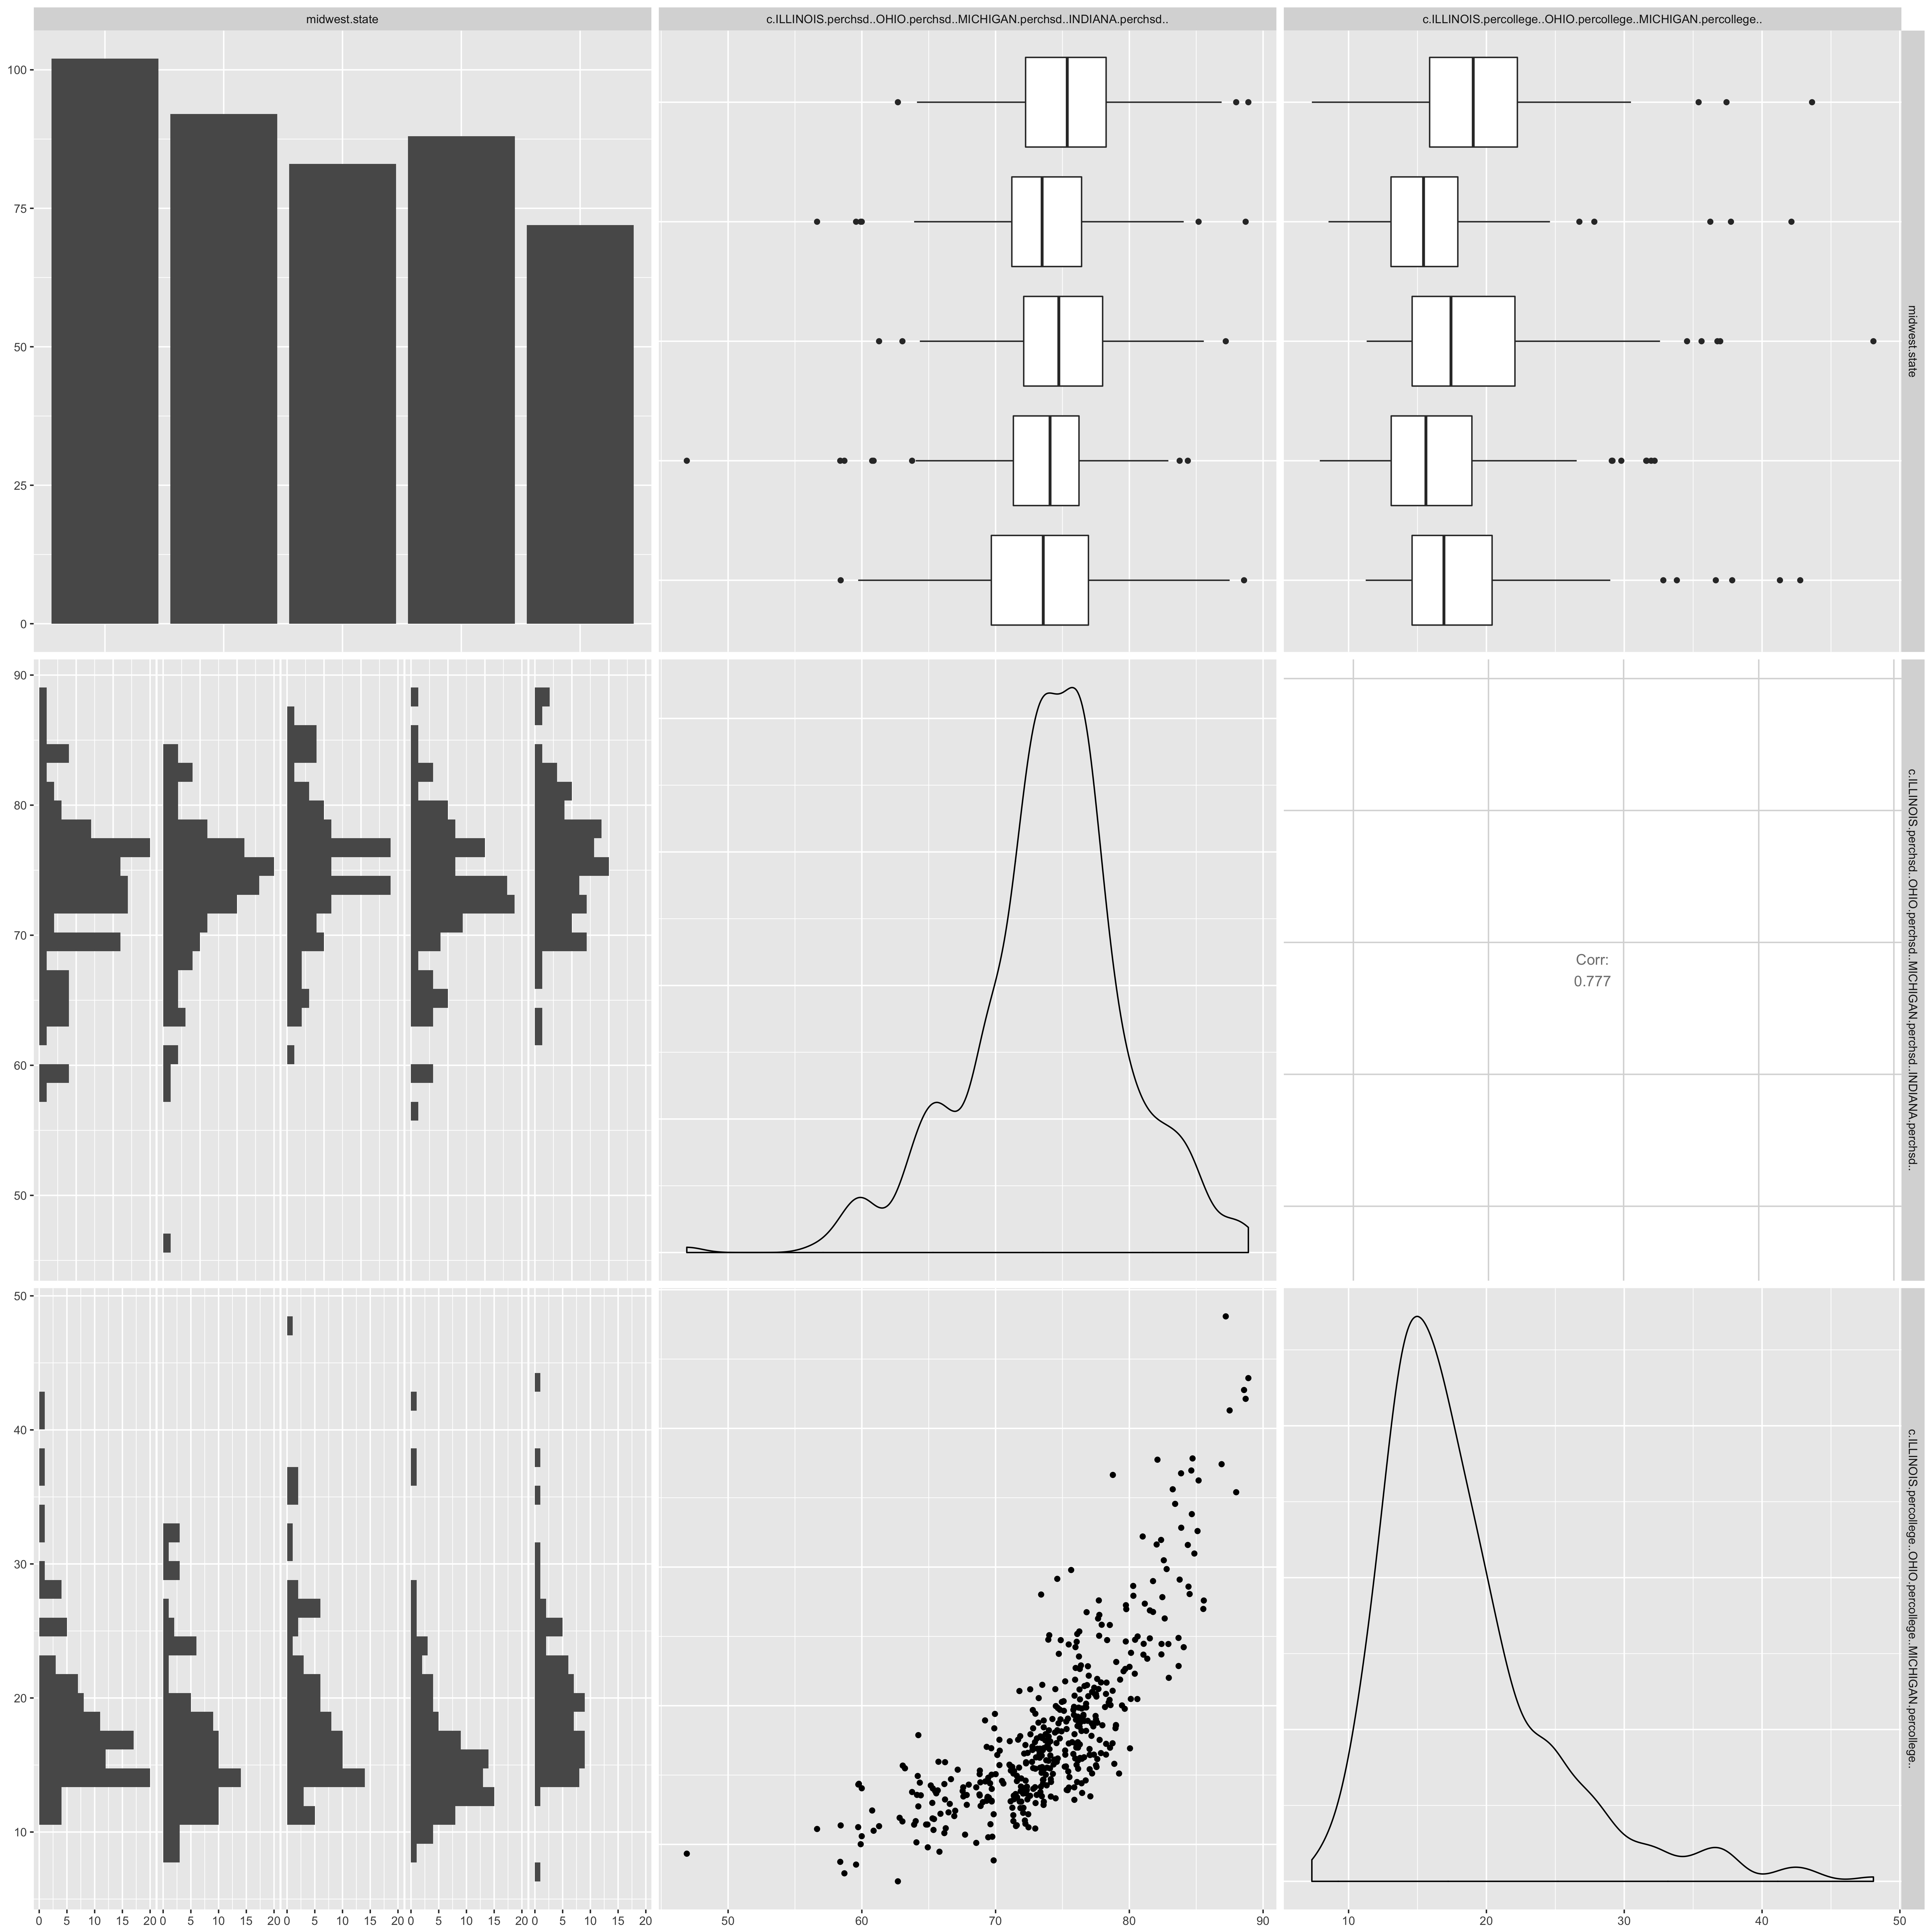
\includegraphics[width=1\textwidth]{pairplot_question2.png}
 \caption{Combined pair-wise plot}
\label{question2}
\end{figure}

Firsly let's analyze the histogram of the states. It represents the number of counties in each state. We can order increasingly as WI < MI < OH < IN < IL. Hence Wisconsin has less counties than Illinois.

Now we can observe the densities of the distributions the percentage of people with High School diploma and the percentage of college educated population. It seems that they follow Gamma law with their respective peaks around [72-77] and [14-16].

Secondly, let's analyze the boxplot between the percentage of people with High School diploma and states : 
Since the boxplots show median, we can determine the order between colors :
IL < IN < MI < WI < OH . We can see that the most spread color is IN and the less one is IL but they are all quite the same. We can also notice that all the medians are inferior to $75\%$ except OH but all superior to $70\%$  and that all third quartiles are positionned lower than $80\%$ ($75\%$ of samples have a percentage of high school diploma inferior to $80\%$). The most important element in boxplots are often outliers here we can see that there is no big differences. IN has the fewer ouliers, MI has the most outliers and the minimum value whereas the maximum value is approximately reached by 3 states over 5. These high values of percentage of high school diploma can be explained by the fact that school is mandatory until 16, 17 or 18 years depending on the state.

Thirdly, let's analyse the boxplot between the percentage of college educated population and states : 
The order between states is the same : IL < MI < IN < WI < OH 
The most spread color is again WI and the less one IL. There are no disjoint values.
We can also notice that all the medians are inferior to $20\%$ and that all third quartiles are positionned lower than $30\%$.
OH has the fewest outliers important whereas IN has the most (they have approximately all the same numbers of outliers between 3 and 6). The maximum value is reached by WI.

Finally, let's analyse the relationship between the percentage of college educated population and the percentage of people with High School diploma : 
As the correlation factor is 0.72, it leads us to the conclusion that those two variables are not strongly related.
The scatter plot does not show a linear model but we can see that the curve is increasing. The observation that when the percentage of people with High School diploma is high, the percentage of college educated people is high too seems logical since High School is required to go to college most of the time.



\section{Comparison of Visualization Techniques}
\paragraph{Boxplot}
Histograms, box plots and qqplots are part of the chart aid category but we will see in this section that they are designed for different uses.
A box plot known also as box-and-whisker plot, is a chart where the main statistical parameters of a data set are graphically represented. 
Those values are the first quartile, the third quartile, the minimum and maximum values and the median. Let's take an example to visualize the construction of the box plots and the meaning of quartiles and median.

\begin{Schunk}
\begin{Sinput}
> library("ggplot2")
> values = floor(runif(100, min=10, max=100))
> values = c(values,150,350,200,1,2)
> val = data.frame(values)
> ggplot(val, aes("",values)) +
+ geom_boxplot() +
+ coord_flip() 
\end{Sinput}
\end{Schunk}

\begin{figure}[!ht]
\centering
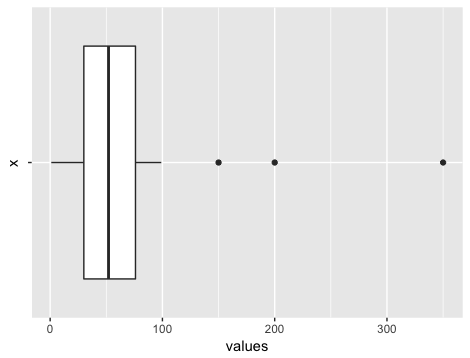
\includegraphics[width=.5\textwidth]{question3.png}
 \caption{Boxplot example}
\label{boxplot}
\end{figure}

The steps that allows us to built this chart are :
\begin{enumerate}
  \item Sort the list's values.
  \item Compute the median of the numbers' serie which is the number wich shares the serie in two parts numerically equal (as much data before and after the median).
  \item Find the first and third quartile. The first quartile being the median of the first part of the serie before the global median, and the third quartile being the median of the second part after the global median. The distance between those two quartiles is called Interquartile range (IQR).
  \item Two other statistical parameters need to be taken into account, they are : $Q_1-1.5 IQR$ and $Q_3 + 1.5 IQR$. Indeed, those two values are the extreme point of the whiskers.
  \item The outliers point outside the boxplot and the whiskers are above the values computed previously.
\end{enumerate}

Hence in our example, we can see that the horizontal axis displays values. 
A vertical line join the summary numbers within the quadrant and a box is drawn around the three quartiles. A line is drawn from the left box edge to the minimum whereas the right line is drawn until $Q_3 + 1.5 IQR$ which is not the maximum that's why we can visualize the three outliers.

\paragraph{Comparison between histogram and boxplot}
A much commconly used chart is the histogram. It graphically displays the frequencies of a data set. Similar to a bar chart, a histogram plots the frequency, or raw count, on the Y-axis and the variable being measured on the X-axis.

As we want to compare those two charts, let's determine the pros and cons of each one in table \ref{table}.

\begin{table}[!ht]
\begin{center}
\caption{Pros and Cons of Histograms and Boxplots}
\label{table}
\begin{tabular}{|l|l|l|l|}
\hline
\multicolumn{2}{|c|}{\textbf{Histogram}}                                     & \multicolumn{2}{c|}{\textbf{Boxplots}}                                     \\ \hline
\multicolumn{1}{|c|}{{\ul \textit{Advantages}}}                               & \multicolumn{1}{c|}{{\ul \textit{Drawbacks}}}                              & \multicolumn{1}{c|}{{\ul \textit{Advantages}}}                             & \multicolumn{1}{c|}{{\ul \textit{Drawbacks}}}                             \\ \hline
\begin{tabular}[c]{@{}l@{}}Summarize \\ numeric data \\ by showing \\ the values' \\ distribution\end{tabular}                                          & \begin{tabular}[c]{@{}l@{}}Unable to visualize the \\ dataset summary\end{tabular} & \begin{tabular}[c]{@{}l@{}}Summarize the statistical \\ parameters of a dataset\end{tabular}                                                 & \begin{tabular}[c]{@{}l@{}}The dataset \\ presenting \\ a modal behaviour \\ would look normal \\ since the \\ values would \\average \\ one another.\end{tabular} \\ \hline
\begin{tabular}[c]{@{}l@{}}Adequated to wide \\ variances among \\ the observed \\ frequencies \\ for a dataset \\ =\textgreater allows to detect \\ recurring groups of \\ numbers \\ (commonly called \\ modes)\end{tabular} & \begin{tabular}[c]{@{}l@{}}The width of the bins \\ influences the level of \\ detail. \\ Very narrow bins \\ =\textgreater hard to draw conclusions \\ Very wide bins \\ =\textgreater lose information due \\ to overly \\ aggressive smoothing.\end{tabular} & \begin{tabular}[c]{@{}l@{}}Provide informations of \\ the datas symmetry and \\ skew-ness and the \\ presence of outliers.\end{tabular}   & \begin{tabular}[c]{@{}l@{}}Original data is not \\ clearly shown in \\ the box plot.\\ Mean cannot be \\ identified in a\\ box plot.\end{tabular}               \\ \hline
\begin{tabular}[c]{@{}l@{}}Identify several\\ features :\\ Mean value = Average \\ across all the blocks\\ Maximum value \\ = Highest block\\ Minimum value\\  = Lowest block\end{tabular}                                 & \begin{tabular}[c]{@{}l@{}}Impossible to extract \\ the exact amount of \\ "input" in the histogram \\ unless it is a frequency \\ histogram.\\ Histograms are often \\ considered inconvenient \\ when comparing multiple \\ categories\end{tabular}           & \begin{tabular}[c]{@{}l@{}}Able to compare \\ several datasets on \\ the same graph by \\ using a boxplot for \\ each category.\end{tabular} & \begin{tabular}[c]{@{}l@{}}Hide many \\ distributions \\ details and \\ emphasize \\ the tails \\ distribution.\end{tabular}                                    \\ \hline
\end{tabular}
\end{center}
\end{table}

\paragraph{Use of the 3 charts : Histogram, Boxplot and QQ-plot}

Finally, a last chart can be examine as the two previous ones. Quantile-quantile plots, also known qq-plots, can be used to compare two datasets, one nmay be sampled from a fixed distribution. They take the form of scatter plots of the quantiles of one dataset against the quantiles of the other dataset. We can draw several conclusions from the shape of the qq-plot. For example, if it's a stright line with a slope of 1 and passing through the origin then the two datsets have the same distribution, if it does not pass through the origin then the two datasets will have the same shape and spread but will be shifted from one another.


\begin{itemize}
  \item When a set of data includes a categorical variable and one or more continuous variables, you will probably be interested to know how the values of the continuous variables vary with the levels of the categorical variable.
Boxplots should not be used when the sample size is small because if only 11 values are present in the dataset and we sort them, to share these datas into 4 equally parts would not be meaningful and it would be difficult to draw conclusion on any statistical parameters. So boxplots should be used for large samples. The current use is to test is there are outliers present in the data. Outliers and skew-ness show the violation of the normality's assumption
  \item Histograms show the distribution of a single numeric variable. They provide more information about the distribution of a singlegroup than boxplots do, at the expense of needing more space. Histogram are best too for large samples. Indeed the choice of the width bin cans be wiser hence give an idea of the shape of the smooth distribution : histogram gives a rough idea of wether or data follows the assumption of normality.
  \item Through the properties quoted above, QQ-plots can be used to determine quickly the analytical nature of a distribution as if it's normal or not. We can also have a direct information on the number of observation which is impossible with boxplots for example.
\end{itemize}


\section{Random Scatterplots}

We generate two sets of N random uniformly distributes values and we increase the number of points N displayed on the scatter plots.

\begin{figure}[!ht]
\centering
\begin{tabular}{ccc}
	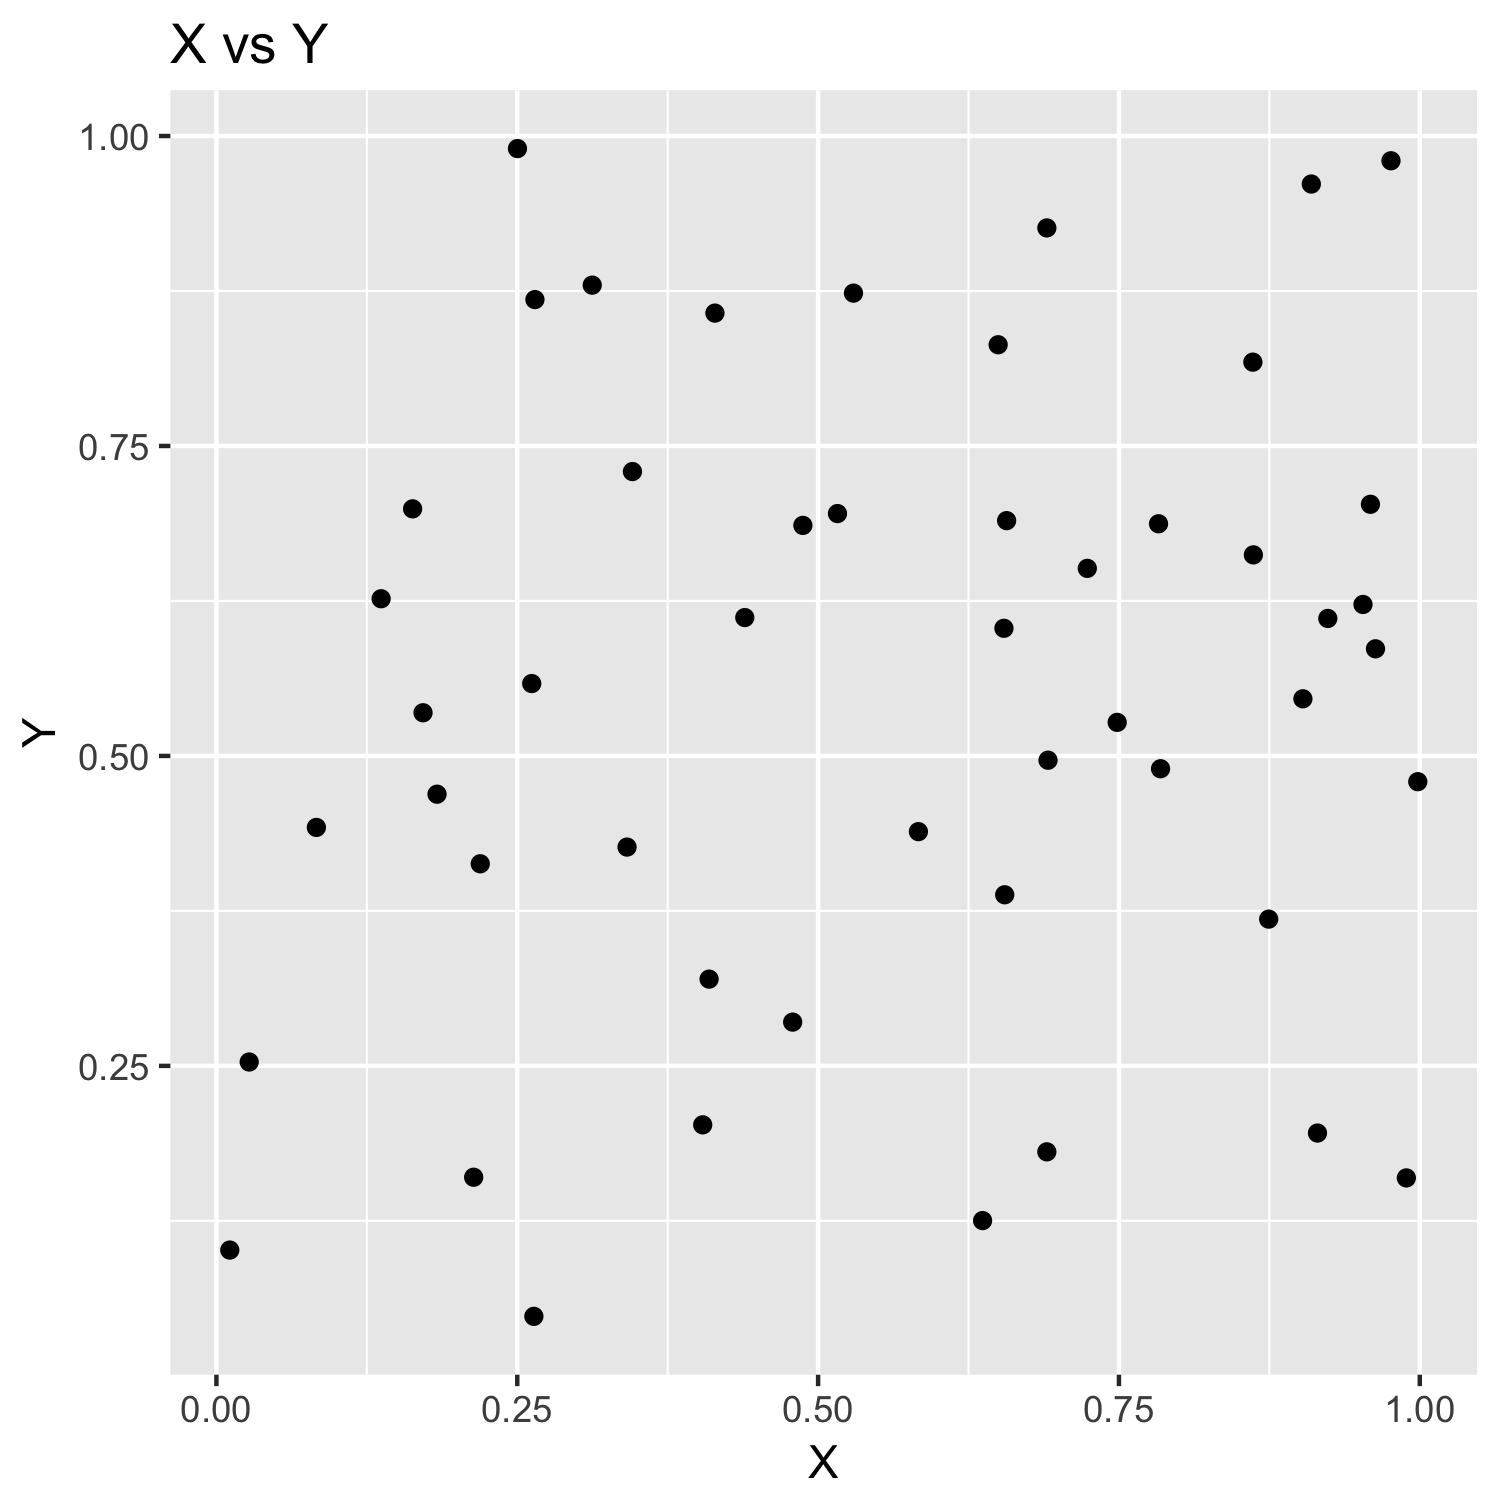
\includegraphics[width=.3\textwidth]{first_plot}&
	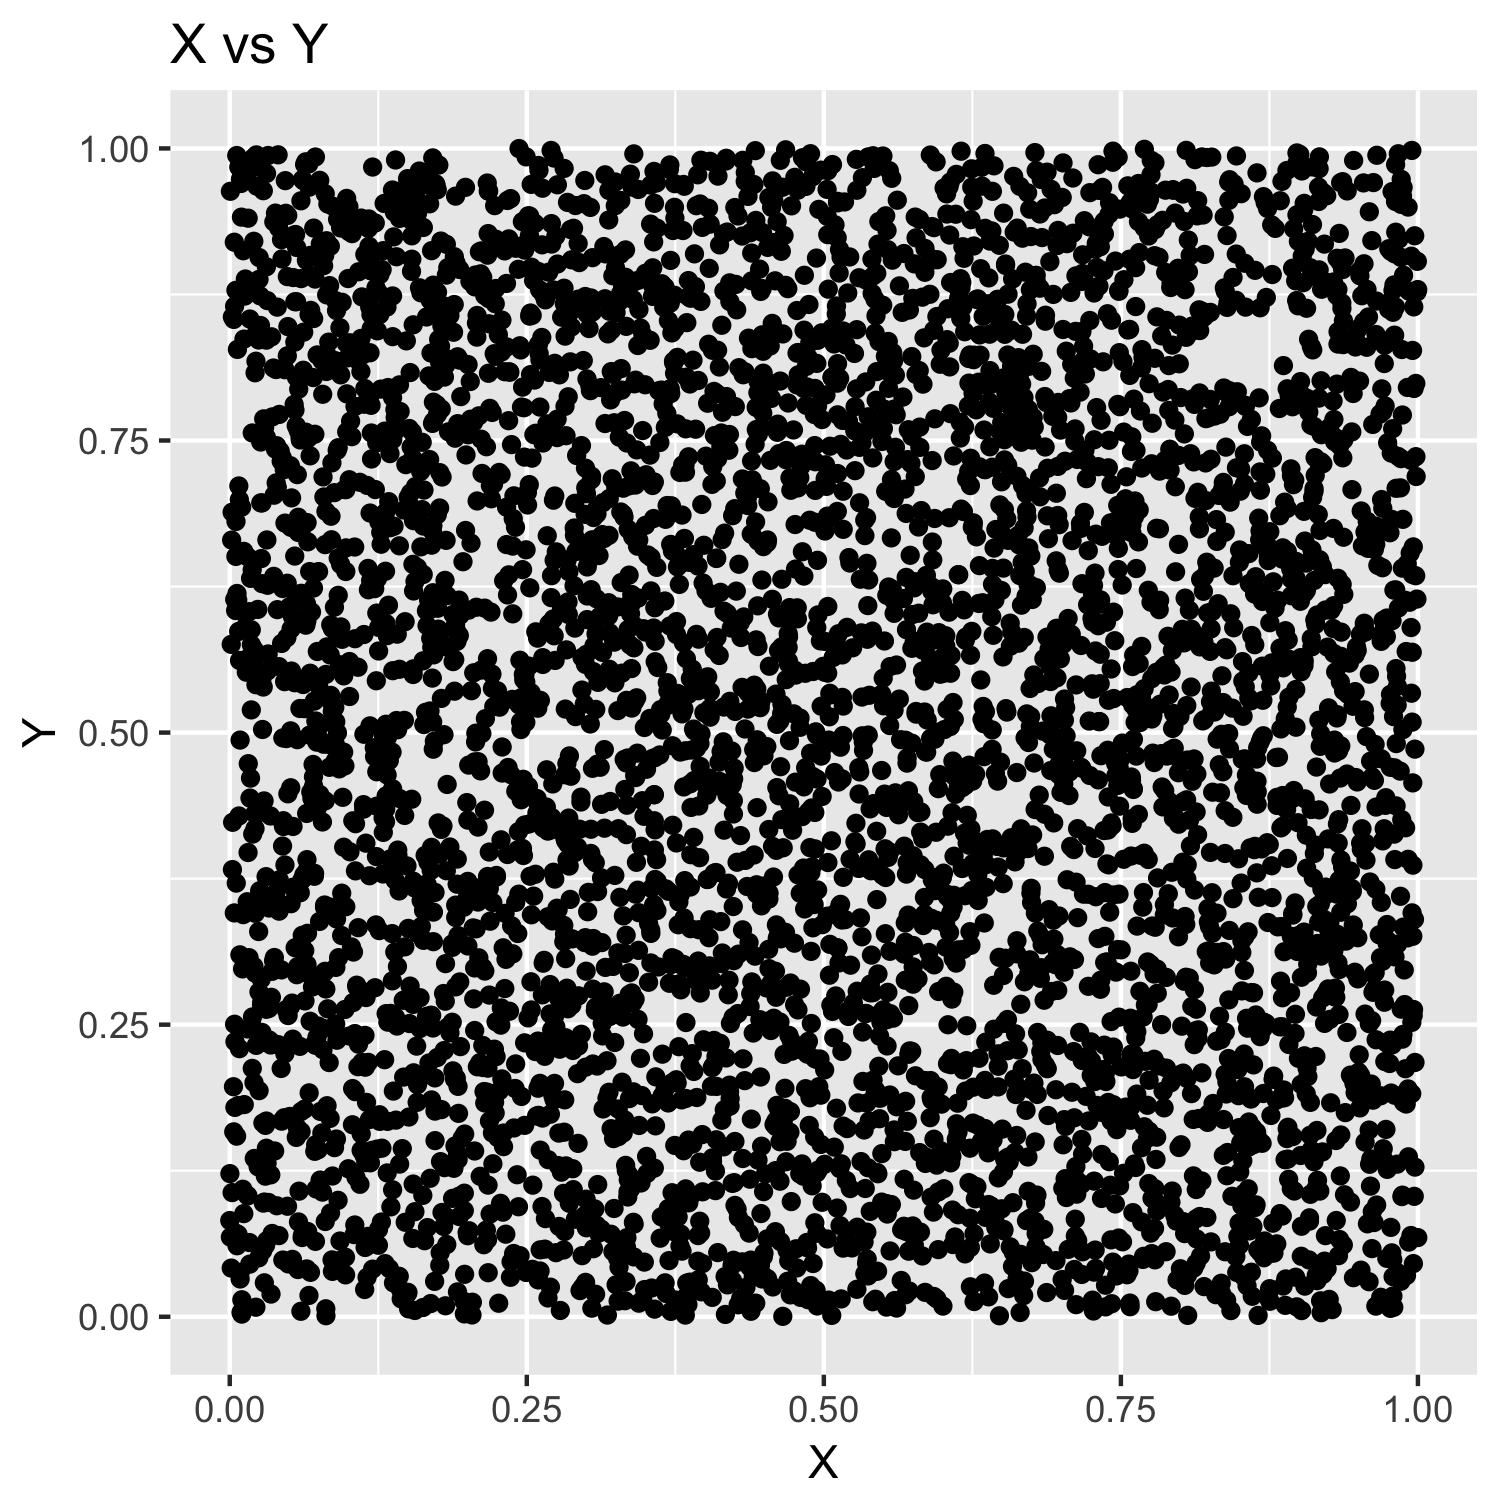
\includegraphics[width=.3\textwidth]{last_plot3}&
	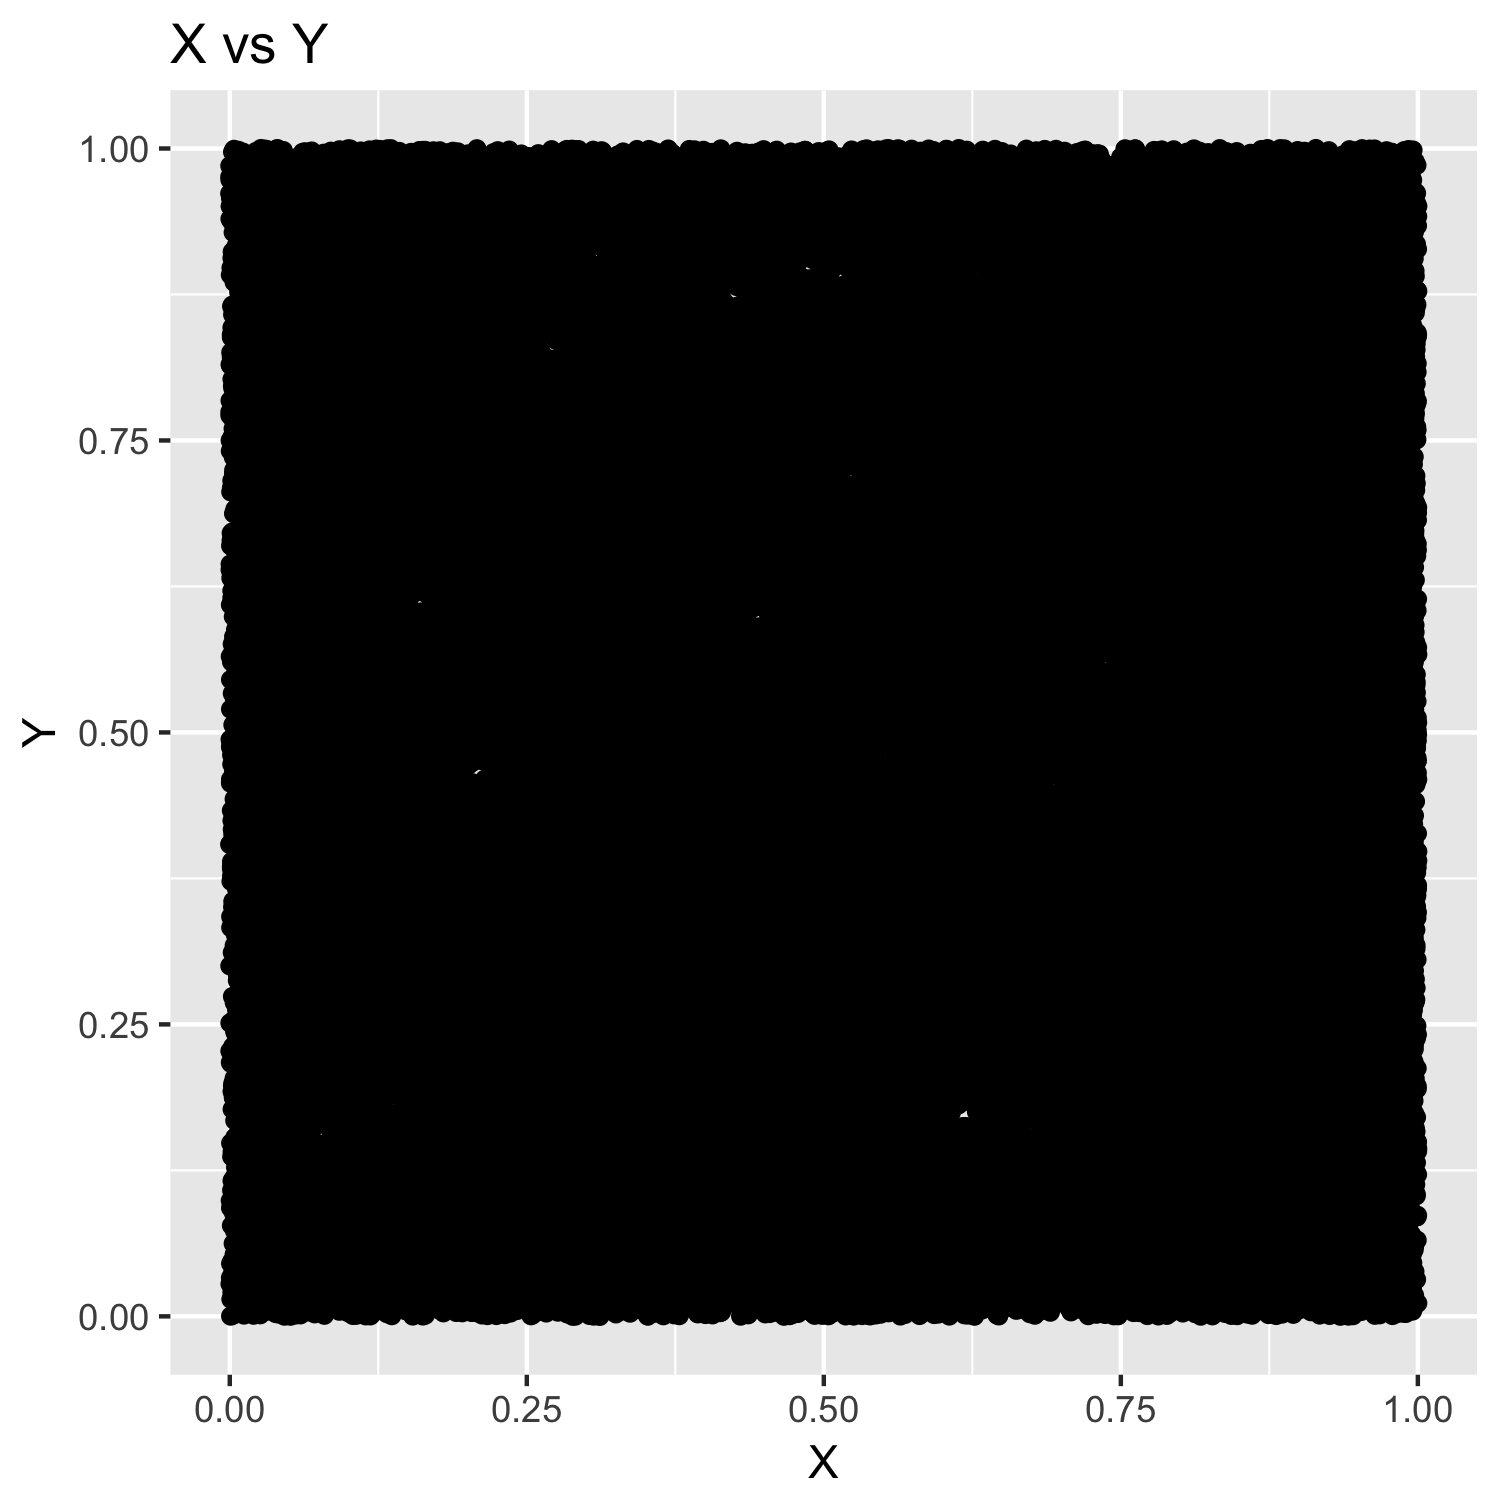
\includegraphics[width=.3\textwidth]{last_plot2}\\
	a&b&c\\
\end{tabular}
\caption{\textit{a}. Scatter plot for N = 50. \textit{b}. Scatter plot for N = 5000. \textit{c}. Scatter plot for N = 50000.}
\label{scatter_plot_format}
\end{figure}
The figure \ref{scatter_plot_format} allows us to visualize the effect of increasing the number of points.
Let's analyse firstly each of the 4 studied formats : 
\begin{itemize}
  \item JPEG format (Joint Photographic Experts Groups) is characterized by the ability to display millions of colors, to process images on 24 bits (16777216 colors), and to compress till $60\% - 75\%$ to obtain an optimal effect. This format is  adequated to fixed image, photos, complex colored images and to shaded images. It's the best image quality available with a great ratio of compression.
  \item PNG format (Portable Network Graphics) provides two formats : PNG8 and PNG24 (the same number of colors as JPEG), it compresses data without loss of data, allows transparency and can be applied on colored background while keeping the original appearance.
  \item PS format (PostScript) storages the file in a vectorial shape wheras JPEG and PNG were matricial format. This file is aimed to impression. This format is a secure way of letting this document available without modification rights. However, it would be better to avoid tranfering this type of file through low speed links via the web.
  \item PDF format (Protable Document Format) has the particularity of keeping the aspect of a document (typographi, position of objects) while being dynamic.
\end{itemize}
In order to compare those formats, we save the size of each file while N is growing.

\begin{figure}[!ht]
\centering
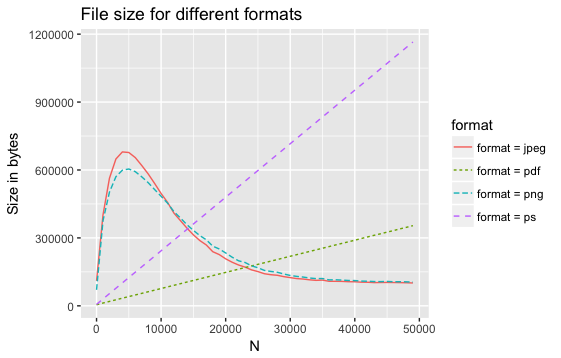
\includegraphics[width=.8\textwidth]{size_file.png}
 \caption{Comparison between four file formats : Postscript, JPEG, PNG and PDF}
\label{size_file}
\end{figure}

The figure \ref{size_file} shows that the size of all format keep growing until $N = 5000$ and while PS and PDF are increasing, PNG and JPEG are decreasing from 5000 to $N \rightarrow \infty$. By analysing slopes, we see that PS and PDF follow linear (growth rate in 0(N)) behaviour with respectively 24 and $7.5$.
The curves for PNG and JPEG show the compression aspect of those formats than can be explained by the fact that after $N = 5000$, it is easier to compress the images since it becomes darker and darker, with more black points than white backgrounds as we can see on the figure \ref{scatter_plot_format}. The growth rate is difficult to determine, although it would seem that the decreasing part follows is in 0(ln(N)). Hence, there is no need of much space to store those images whereas PS and PDF do not overcome compression that's why their size keep growing.

\section{Diamonds}

\paragraph{Distributions}
We will now analyze the distribution of three variables of the dataset diamonds : color, carat and price.
To do so, we will use different tools. Concerning the color variable which is a categorical one, the histogram can't be used since it's not a numerical variable hence bar chart fits well to that type of variable. Carat and price can be represented with histograms.
\begin{figure}[!ht]
\centering
\begin{tabular}{cc}
	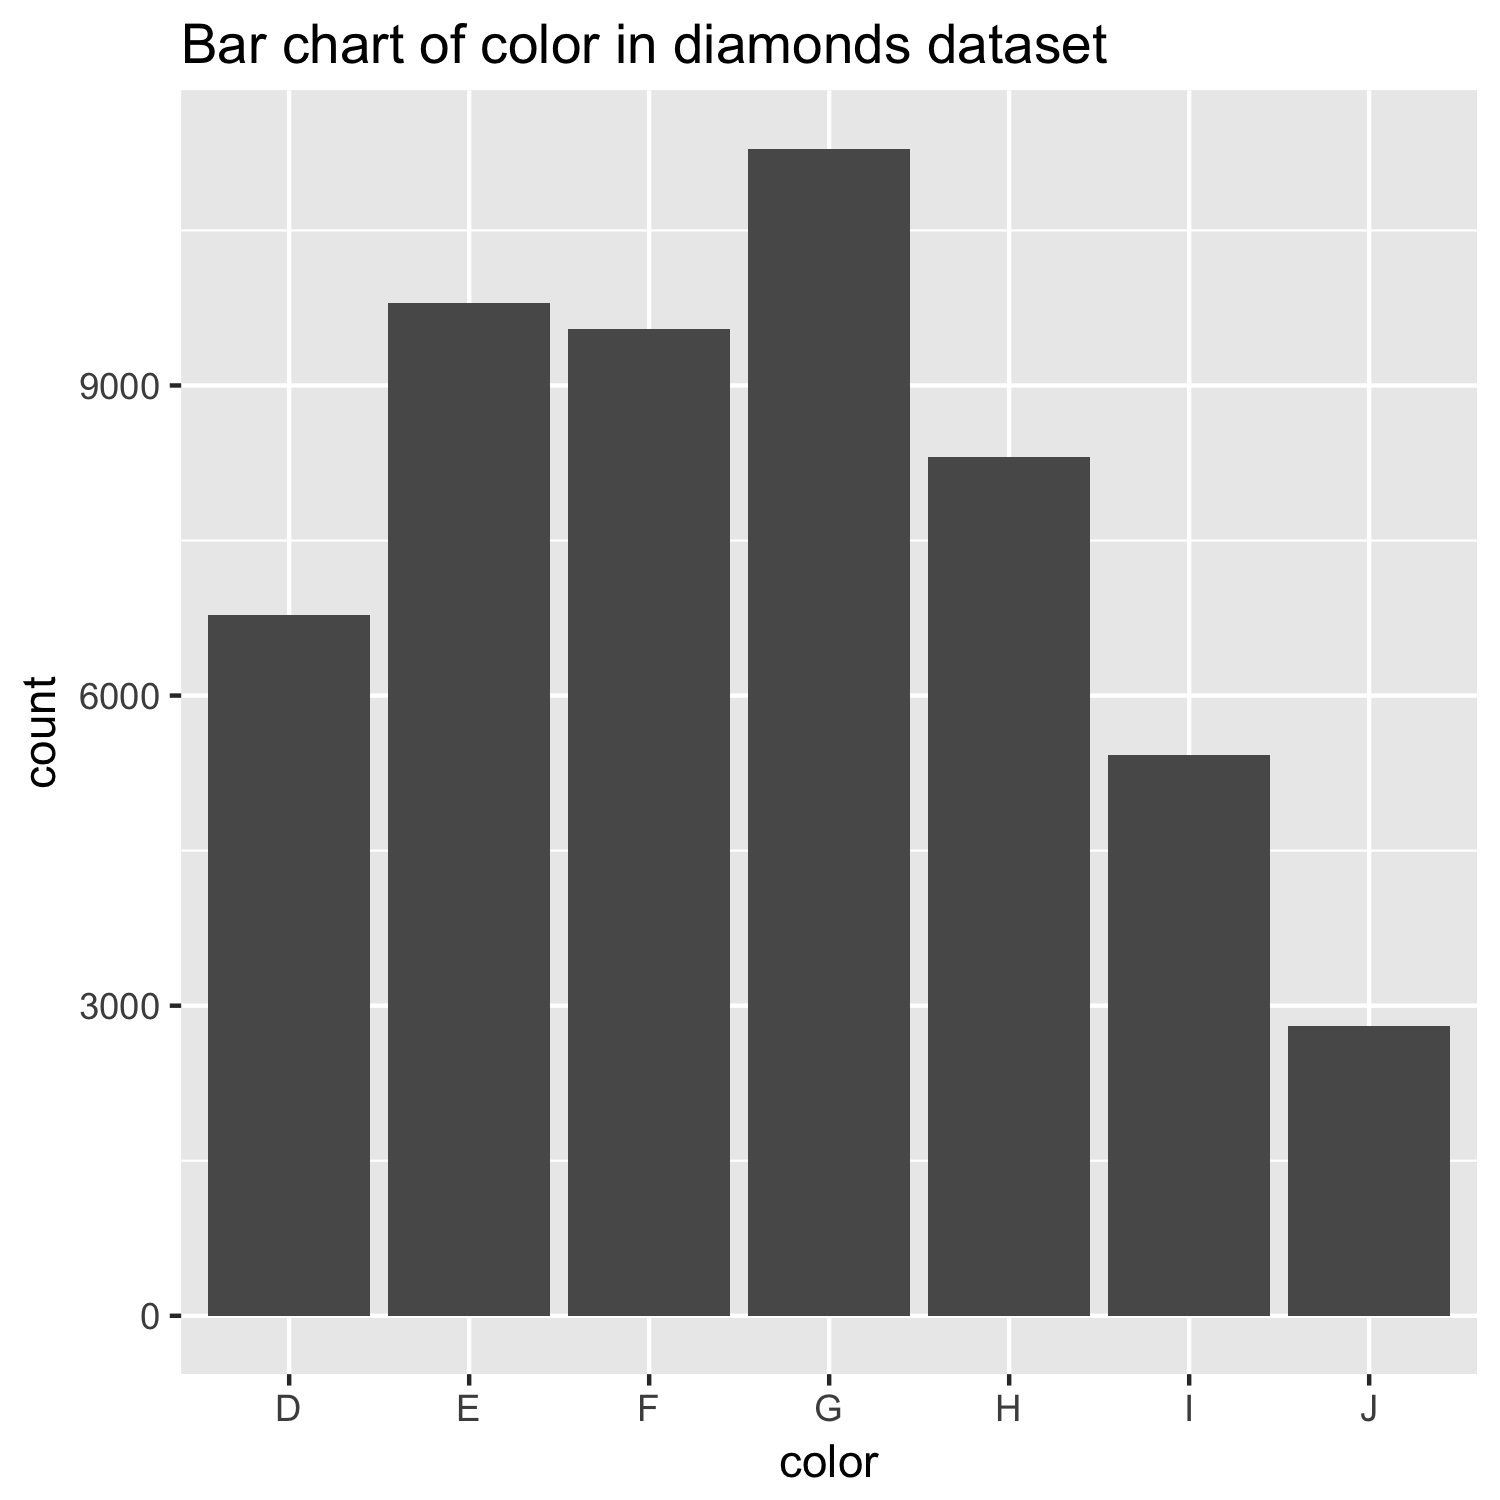
\includegraphics[width=.5\textwidth]{bar_chart_color}&
	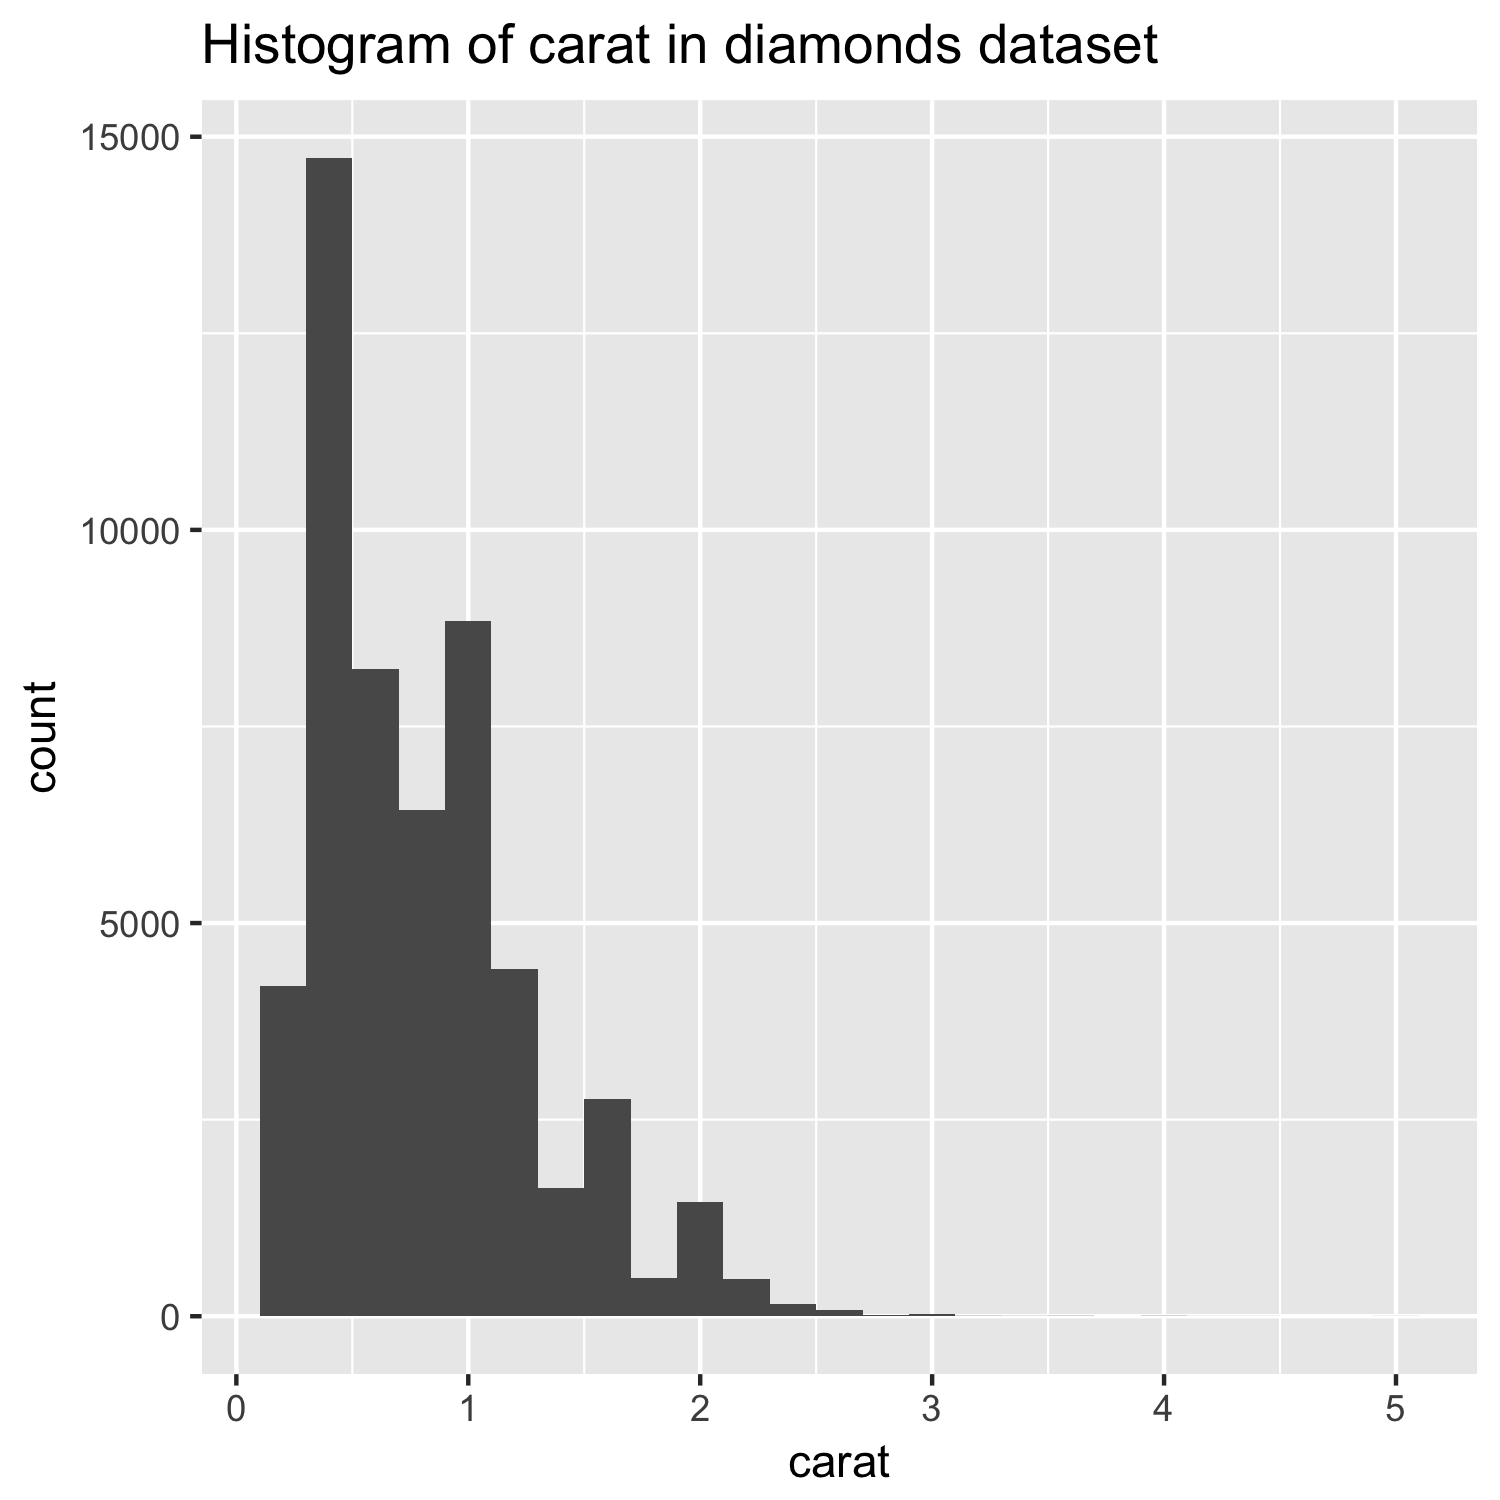
\includegraphics[width=.5\textwidth]{histogram_carat}\\
	a&b\\
	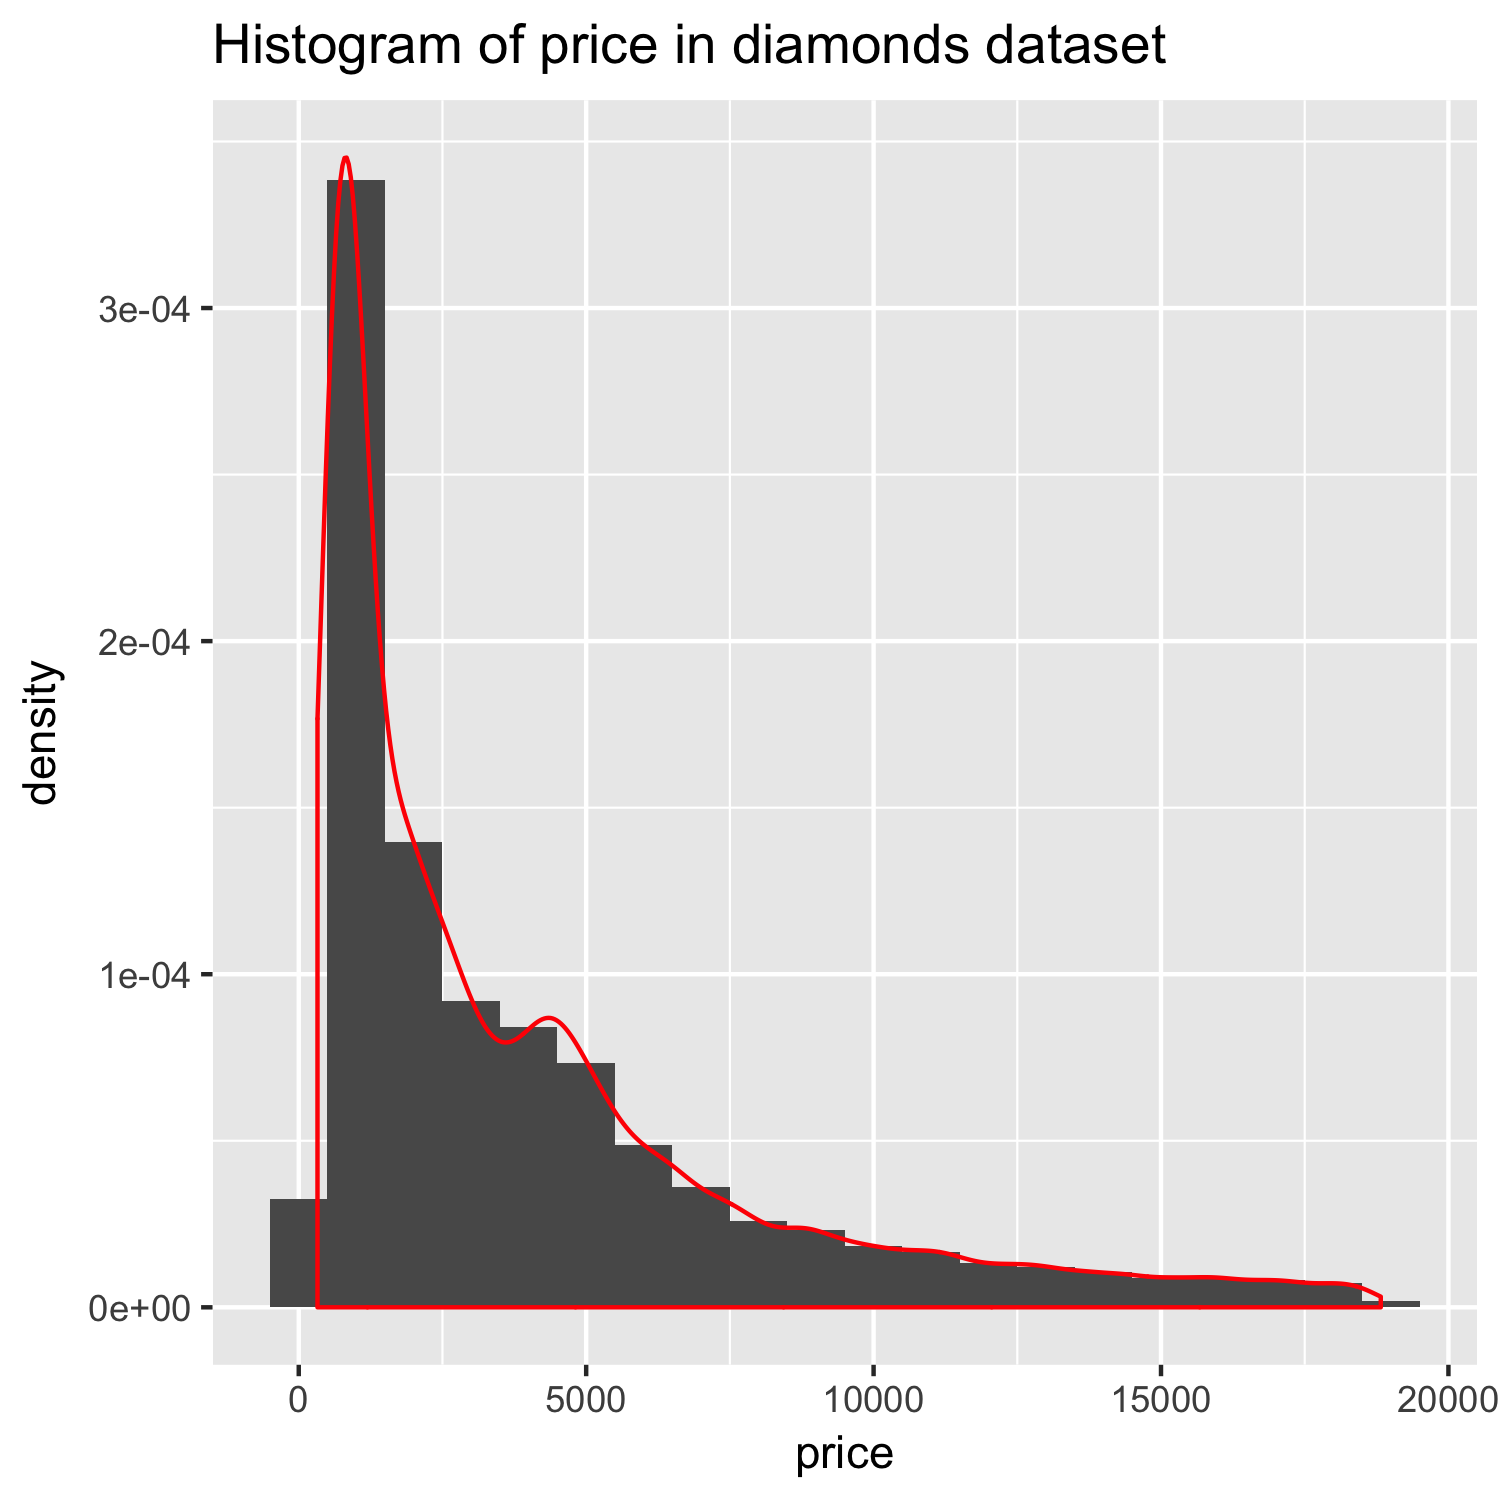
\includegraphics[width=.5\textwidth]{histogram_price}\\
	c\\
\end{tabular}
\caption{\textit{a}. Bar chart for color. \textit{b}. Histogram for carat. \textit{c}. Histogram for price.}
\label{diamonds}
\end{figure}

As we can see on the figure \ref{diamonds}a. ,seven types of color are present with different frequencies. If we wanted to sort their frequency in an increasing order, it would be : J < I < D < H < F < E < G. J can be count less than 3000 whereas G approximately 10000. We can't say much about the distribution.

The figure \ref{diamonds}b. shows the distribution of carat. The choice of binwidth was crucial to be able to see the different peaks present indeed with a bindwidth larger than 0.2, the distribution is smoothed. Hence the remarkable values are around [0.3-0.5] and [0.9-0.11]. As the density didn't seem like any reknown distribution, it was not relevant to present it.

The figure \ref{diamonds}c. shows the distribution of price. 
Once more the binwidth is important to be able to see a suitable graph. The density here allows us to identify a long tail distribution (also known as Paretto dstribution) where it would seem that the parameter k is equal to 2. We can observe a peak at $1000\$$.

\paragraph{Three-way relationship}

In order to analyze the links between price, carat and color, we will insvestigate the three-way relationship. An efficient tool is provided by GGAlly and called ggpairs.

\begin{figure}[!ht]
\centering
\includegraphics[width=0.9\textwidth]{pairplot.png}
 \caption{Combined pair-wise plot}
\label{pairplot}
\end{figure}

We can visualize on the figure \ref{pairplot} that the graphs presented on the diagonal are those explained before. The bar chart of the colors is the same than preciously, the density of price. The density of carat has not been exploited before because of its lack of meaning.
In order to study price and carat vs color, we won't use histograms but boxplots according to our analyze of pros and cons for histograms and boxplot because it is more adequatied to the analysis of the relationship between variables.

Firstly, let's analyze the boxplot between carat and color : 
Since the boxplots show median, we can determine the order between colors :
E < D < G < F < H < I < J. We can see that the most spread color is I and the second one is J. We can observe that the box D and E are similar, F and G are also similar. We can also notice that all the medians are inferior to 1.2 and that all third quartiles are positionned lower than 1.5 ($75\%$ of samples have a carat size inferior to 1.5). The most important element in boxplots are outliers hence we can observe that the difference between colors are in the number and positions of those. J has the fewer ouliers but has the highest maximum. F and G has lowest maximum but a lot of outliers.

Secondly, let's analyse the boxplot between price and color : 
The order between colors is the same : E < D < G < F < H < I < J.
The most spread color is again J and the second one I. Contrary to the previous analaysis, F and G are not similar, D and E neither. 
We can also notice that all the medians are inferior to 5000 and that all third quartiles are positionned lower than 10000 (all are inferior 7500 except J).
E has the number of outliers the most important and J the fewest (I has approximately the same number of outliers than J). The maximum price is the same for all colours which is really different from the size of carat. 

\begin{figure}[!ht]
\centering
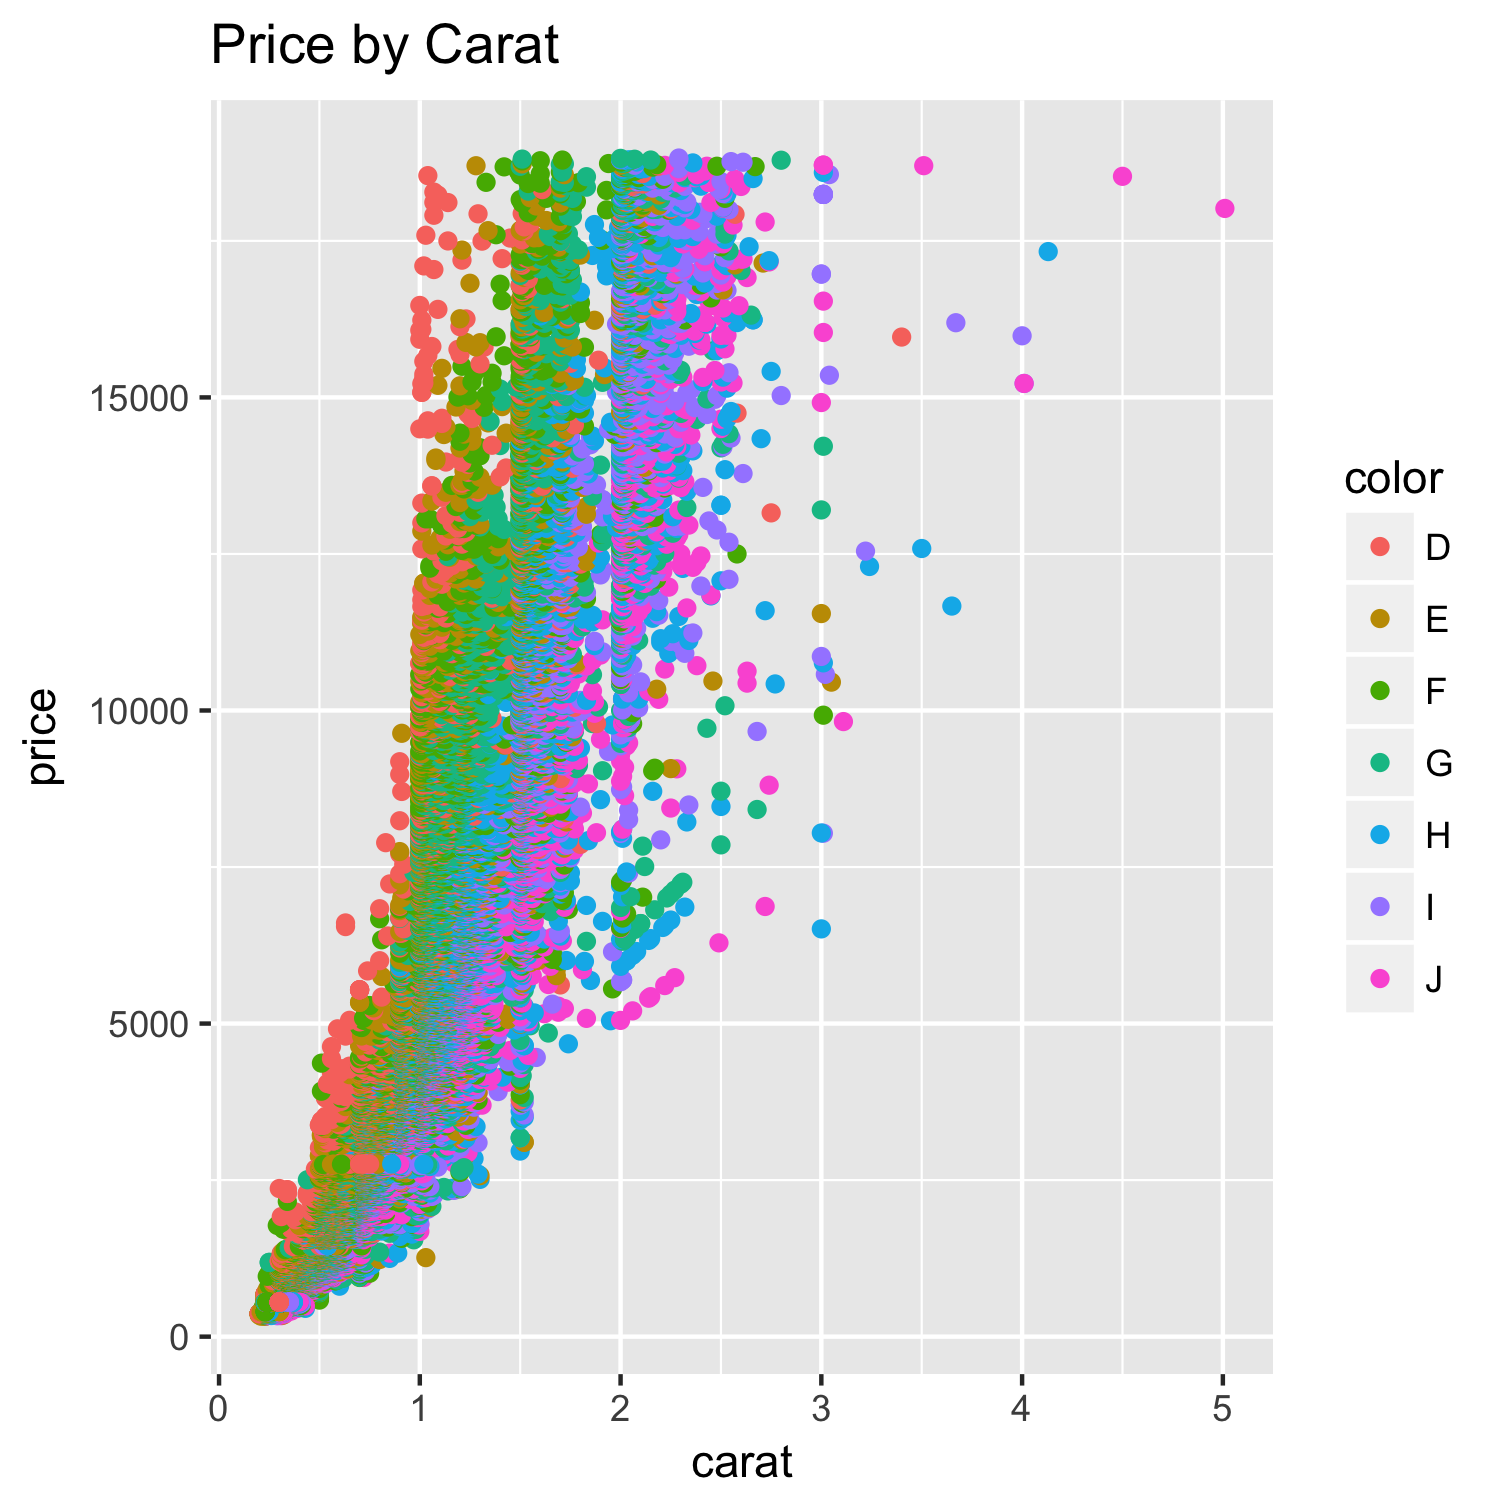
\includegraphics[width=.5\textwidth]{pricebycarat.png}
 \caption{Relationship between price and carat}
\label{pricebycarat}
\end{figure}

Finally, let's analyse the relationship between price and carat : 
The correlation factor is 0.922 which means that the relationship is linear.
The scatter plot of figure \ref{pricebycarat} shows that carat evolves approximately linearly according to price. This observation fits to the linear model that follows our scatter plot. What might be surprising is the absence of mix in the colours, each one has a specific range for carat and price. Hence the slope that we can easily visualize are increasing such that J < I < H < G < F < E < D.

\end{document}
